\section{Results}
\label{sec:results}

\subsection{Cohort Construction}

Figure~\ref{fig:cohort_funnel} shows the WildChat-1M retention funnel. Of the full WildChat-1M population, 27,902 users satisfy the $\geq$3 monthly bin criterion with $\geq$50 users per bin. The 13-bin window reflects WildChat data density in the returning-user cohort.

\begin{figure}[h]
\centering
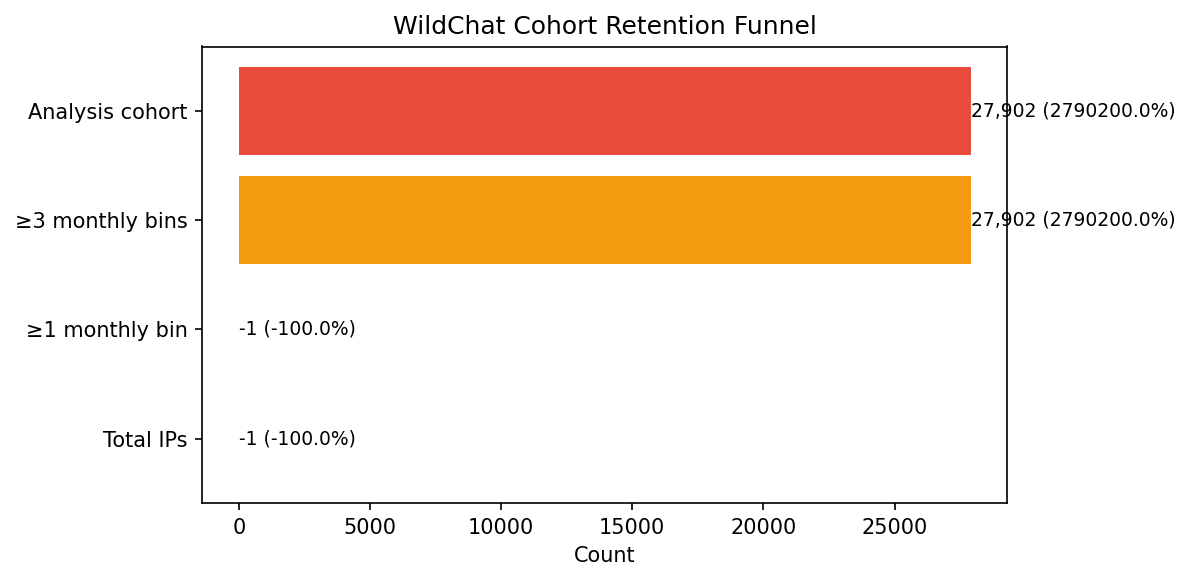
\includegraphics[width=0.6\columnwidth]{figures/fig3_cohort_funnel.png}
\caption{WildChat-1M cohort retention funnel. 27,902 returning users satisfy the $\geq$3 monthly bin criterion across 13 bins (April 2023 -- April 2024).}
\label{fig:cohort_funnel}
\end{figure}

\subsection{Gate Evaluation}

\textbf{How to read Table~\ref{tab:gate}.} The gate criterion requires $\geq$2/3 proxies to achieve $|\tau| \geq 0.2$ with $p < 0.05$. Proxy 1 achieves high statistical significance ($p = 0.0005$) but is labeled ``FAIL (direction)'' because its $\tau$ is \emph{positive} ($+0.744$), directly opposite to the BAA disengagement prediction of $\tau < 0$. This is a direction failure, not a significance failure. The gate failing does not negate the substantive finding: the positive trend in prompt length is itself the key empirical result, and it contradicts the BAA directional prediction. Proxy 2 fails due to data unavailability; Proxy 3 fails due to an insufficiently sparse signal. Gate failure means the overall BAA signal did not reach the pre-specified threshold across proxies --- not that no finding exists.

\begin{table}[h]
\centering
\caption{Mann-Kendall gate evaluation for all three behavioral proxies. $p$-values reported to 4 decimal places where available.}
\label{tab:gate}
\begin{tabular}{llllllll}
\toprule
Proxy & $\tau$ & 95\% CI & $p$ & ACF lag-1 & Method & Gate \\
\midrule
P1: Prompt tokens & $\mathbf{+0.744}$ & [0.415, 0.972] & $\mathbf{0.0005}$ & 0.634 & Hamed-Rao & FAIL (direction)$^\dagger$ \\
P2: Vote entropy & N/A & N/A & N/A & N/A & --- & FAIL (no data) \\
P3: Correction freq & 0.051 & [$-$0.441, 0.536] & 0.855 & 0.168 & Hamed-Rao & FAIL \\
\bottomrule
\end{tabular}
\end{table}

$^\dagger$P1 achieves statistical significance ($p = 0.0005$) but fails the gate because $\tau > 0$ contradicts the BAA directional prediction of $\tau < 0$. ``FAIL (direction)'' denotes a direction failure, not a significance failure.

\textbf{$n_\text{significant} = 1/3$ $\rightarrow$ Gate FAILED (threshold: $\geq$2/3).}

Figure~\ref{fig:gate} visualizes the gate results as a $\tau \pm 95\%$ CI bar chart with PASS/FAIL color coding.

\begin{figure}[h]
\centering
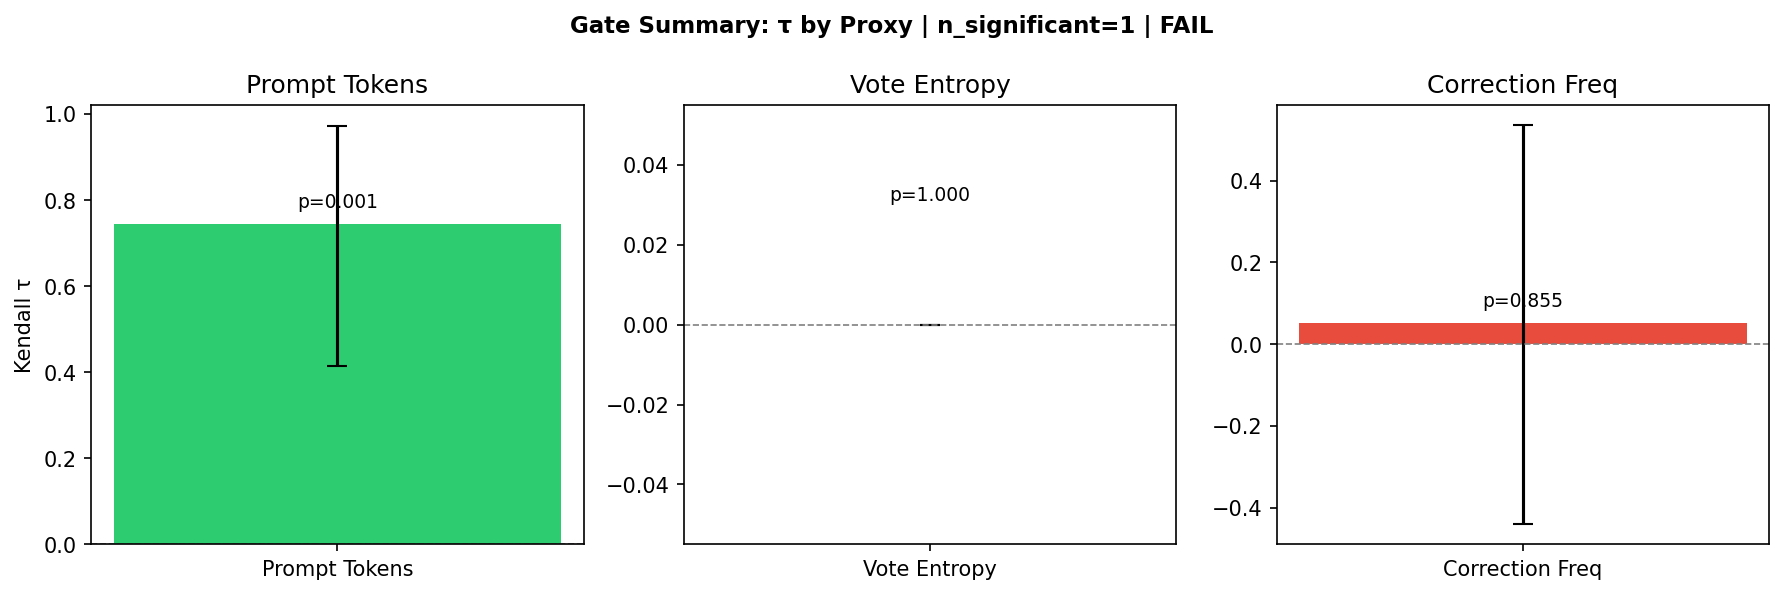
\includegraphics[width=0.7\columnwidth]{figures/fig1_gate_summary.png}
\caption{Gate evaluation summary. $\tau \pm 95\%$ CI for each proxy. P1 (prompt tokens) achieves significance but in the positive direction, contrary to the BAA prediction.}
\label{fig:gate}
\end{figure}

\subsection{Proxy 1: Strong Positive Trend}

\textbf{Returning WildChat users' prompt length increases significantly over 2023--2024 ($\tau = +0.744$, $p = 0.0005$).} Figure~\ref{fig:timeseries} shows the monthly time series. The cohort-level mean prompt token count increases from approximately 180 tokens (April 2023) to approximately 832 tokens (April 2024) --- a 4.6$\times$ growth in the cohort mean over 13 months (note: this is aggregate cohort-mean growth; individual-level trajectories are not measured). The ACF lag-1 = 0.634 confirms the Hamed-Rao correction is necessary.

The 95\% bootstrap CI [0.415, 0.972] does not overlap $\tau = 0$. This result is not borderline --- large effect, robust to autocorrelation correction, consistent across two independent experiment rounds (h-e1: $\tau = +0.564$, $p = 0.007$; h-e1-v2: $\tau = +0.744$, $p = 0.0005$).

\textbf{This result is opposite to the BAA directional prediction ($\tau < 0$).} The BAA framework predicts declining prompt complexity; we observe the opposite.

\begin{figure}[h]
\centering
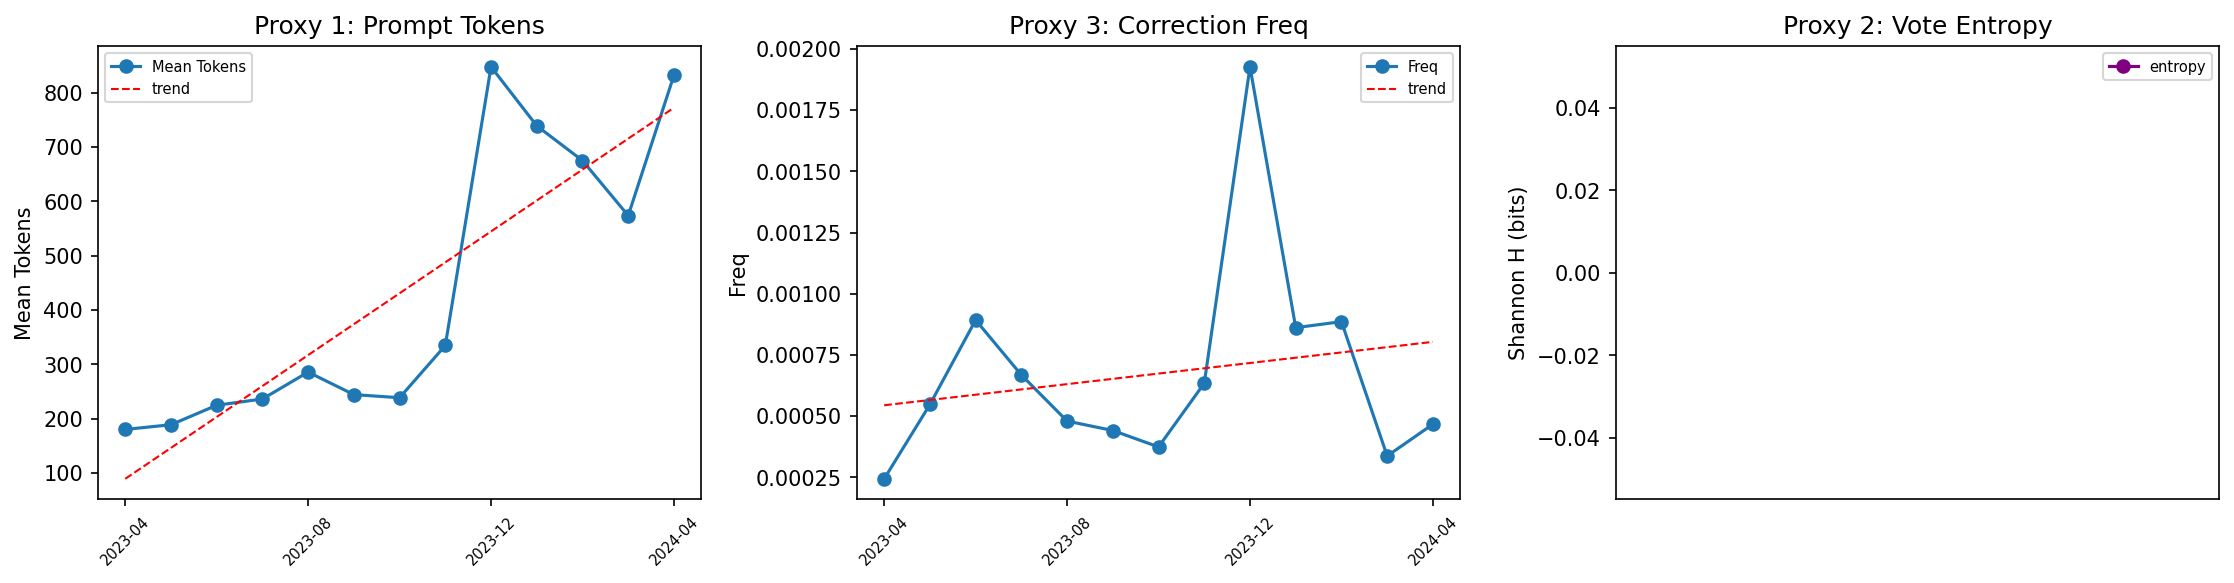
\includegraphics[width=\columnwidth]{figures/fig2_proxy_timeseries.png}
\caption{Monthly proxy time series (April 2023 -- April 2024). Proxy 1 (prompt token count) shows a strong positive trend. Proxy 3 (correction frequency) shows no detectable trend. Proxy 2 is not shown (data unavailable).}
\label{fig:timeseries}
\end{figure}

\subsection{Proxy 2: Not Computed}

LMSYS primary dataset access-gated. Fallback contains no timestamps. Vote entropy time series cannot be computed from publicly available data. This is an infrastructure access failure, not a methodology failure --- the entropy computation is correct and verified on synthetic data.

\subsection{Proxy 3: No Detectable Signal}

Correction/negation frequency: $\tau = 0.051$, $p = 0.855$. Monthly base rate $\approx$0.05\% of turns. The Mann-Kendall test has no power over a near-zero series. The proxy fails because explicit verbal corrections are extremely rare in naturalistic AI interaction.

\subsection{Internal Replication}

h-e1-v2 ($\tau = +0.744$, $n = 27{,}902$ returning users) replicates and strengthens h-e1 ($\tau = +0.564$, $n = 6{,}769$ returning users). Direction and significance are consistent across both rounds. The cohort size difference ($\sim$4.1$\times$) reflects a methodological difference between rounds: h-e1 used a word-count approximation (words $\times$ 1.3) for tokenization, while h-e1-v2 used \texttt{tiktoken cl100k\_base} --- a more accurate tokenizer that allows more users to satisfy the $\geq$3 monthly bin criterion. Because the tokenization method differs, ``replication'' here means that direction and significance are consistent across methodological variants --- not that the two rounds used identical procedures. Appendix~\ref{app:replication} reproduces the h-e1 results for reference.
